\documentclass[aspectratio=169]{beamer}

\usetheme{default}
\usecolortheme{dove}

\setbeamertemplate{navigation symbols}{}
\setbeamertemplate{footline}{%
  \hfill{\large\insertframenumber\,/\,\inserttotalframenumber}\hspace{0.8em}\vspace{0.5em}%
}

\definecolor{popblue}{RGB}{52, 101, 164}
\definecolor{sampred}{RGB}{204, 0, 0}
\definecolor{paramgreen}{RGB}{0, 140, 70}
\definecolor{warnred}{RGB}{180, 40, 40}
\definecolor{orange1}{RGB}{220, 120, 0}
\definecolor{violet1}{RGB}{120, 50, 160}
\definecolor{lightbg}{RGB}{245, 245, 250}

\setbeamercolor{frametitle}{fg=popblue}
\setbeamercolor{title}{fg=popblue}

\usepackage{pgfplots}
\usepackage{tikz}
\usetikzlibrary{shapes, arrows.meta, positioning, calc, decorations.pathreplacing, patterns}
\pgfplotsset{compat=1.18}
\usepackage{amsmath, amssymb}
\usepackage{fontenc}

\title{Lecture 4: Fisher Information \& Cram\'er--Rao}
\subtitle{Score Function $\cdot$ Fisher Information $\cdot$ CR Bound $\cdot$ Admissibility $\cdot$ Stein's Paradox}
\date{}

\begin{document}

% ============================================================
\begin{frame}
\titlepage
\end{frame}

% ============================================================
\begin{frame}
\frametitle{Previously, on Lecture 3\ldots}

\begin{center}
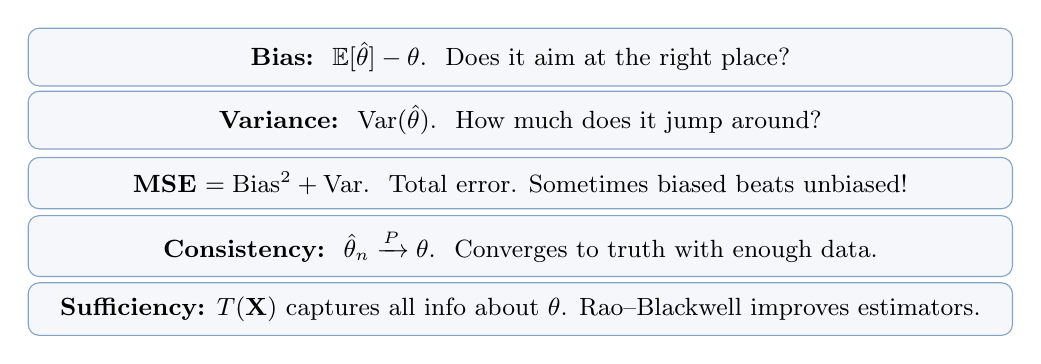
\begin{tikzpicture}[
  sbox/.style={draw=popblue!60, fill=popblue!5, rounded corners=4pt, minimum width=12.5cm, minimum height=0.5cm, align=left, inner sep=5pt, font=\small}
]
  \node[sbox] at (0, 2.4) {\textbf{Bias:} $\;\mathbb{E}[\hat\theta] - \theta$. \;Does it aim at the right place?};
  \node[sbox] at (0, 1.6) {\textbf{Variance:} $\;\text{Var}(\hat\theta)$. \;How much does it jump around?};
  \node[sbox] at (0, 0.8) {\textbf{MSE} $= \text{Bias}^2 + \text{Var}$. \;Total error. Sometimes biased beats unbiased!};
  \node[sbox] at (0, 0.0) {\textbf{Consistency:} $\;\hat\theta_n \xrightarrow{P} \theta$. \;Converges to truth with enough data.};
  \node[sbox] at (0, -0.8) {\textbf{Sufficiency:} $T(\mathbf{X})$ captures all info about $\theta$. Rao--Blackwell improves estimators.};
\end{tikzpicture}
\end{center}

\vspace{0.3cm}
\begin{center}
{\large\textbf{Today:}} Can we quantify the \textbf{best possible} precision?\\[4pt]
Is there a fundamental \textbf{limit} on how good any estimator can be?
\end{center}
\end{frame}

% ============================================================
\begin{frame}
\frametitle{Why Does Lower Variance Matter?}

\small
From Lecture~3: an unbiased estimator \textbf{aims at the right place}. But if the variance is huge, individual estimates are all over the map.

\vspace{0.05cm}
\begin{center}
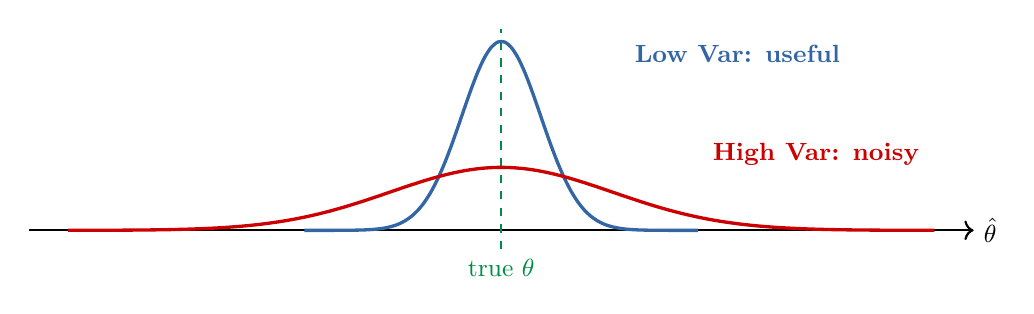
\begin{tikzpicture}[yscale=0.8]
  \draw[thick, ->] (0, 0) -- (12, 0) node[right, font=\small] {$\hat\theta$};
  \draw[dashed, paramgreen, thick] (6, -0.3) -- (6, 3.2);
  \node[below, font=\small, paramgreen] at (6, -0.3) {true $\theta$};

  % Low variance
  \draw[very thick, popblue, smooth, domain=3.5:8.5, samples=60]
    plot (\x, {3*exp(-(\x-6)*(\x-6)/0.5)});
  \node[font=\small\bfseries, popblue] at (9, 2.8) {Low Var: \textbf{useful}};

  % High variance
  \draw[very thick, sampred, smooth, domain=0.5:11.5, samples=60]
    plot (\x, {1.0*exp(-(\x-6)*(\x-6)/4)});
  \node[font=\small\bfseries, sampred] at (10, 1.2) {High Var: \textbf{noisy}};
\end{tikzpicture}
\end{center}

\vspace{-0.1cm}
\pause
\begin{itemize}\setlength{\itemsep}{1pt}
  \item Both estimators are \textbf{unbiased} --- centered on the true $\theta$
  \item But the \textcolor{sampred}{red one} often gives estimates \textbf{far from the truth}
  \item With \textbf{one} sample, you can't tell if you're close or not --- lower variance = higher \textbf{confidence}
\end{itemize}

\vspace{0.05cm}
\centering\textbf{Among unbiased estimators, can we find the one with the \textbf{smallest} variance?}
\end{frame}

% ============================================================
\section{Fisher Information and Cram\'er--Rao}

\begin{frame}
\frametitle{Can We Do Better? The Fundamental Question}

\begin{center}
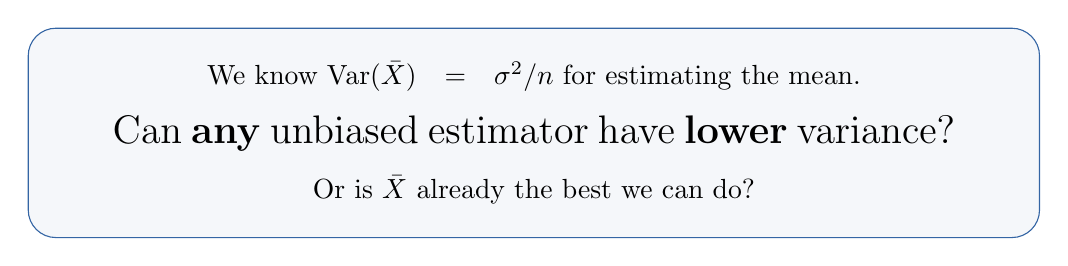
\begin{tikzpicture}
  \node[draw=popblue, fill=popblue!5, rounded corners=10pt, text width=12cm, align=center, inner sep=12pt] {
    We know $\text{Var}(\bar{X}) = \sigma^2/n$ for estimating the mean.\\[8pt]
    {\Large Can \textbf{any} unbiased estimator have \textbf{lower} variance?}\\[8pt]
    Or is $\bar{X}$ already the best we can do?
  };
\end{tikzpicture}
\end{center}

\vspace{0.3cm}
To answer this, we need to measure \textbf{how much information} one observation carries about $\theta$.

\vspace{0.2cm}
\begin{center}
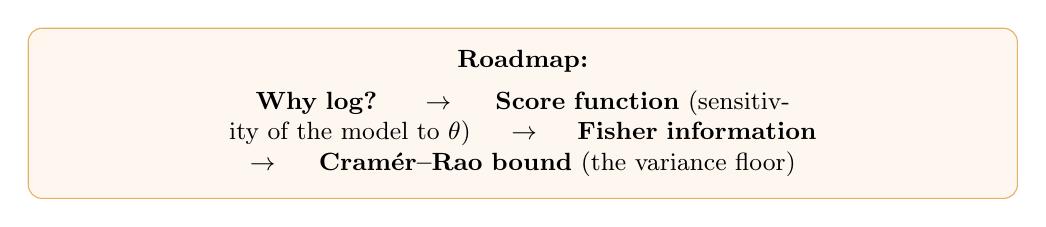
\begin{tikzpicture}
  \node[draw=orange1!60, fill=orange1!6, rounded corners=5pt, text width=12cm, align=center, inner sep=8pt, font=\small] {
    \textbf{Roadmap:}\\[4pt]
    \textbf{Why log?}
    $\;\to\;$ \textbf{Score function} (sensitivity of the model to $\theta$)
    $\;\to\;$ \textbf{Fisher information}\\
    $\to\;$ \textbf{Cram\'er--Rao bound} (the variance floor)
  };
\end{tikzpicture}
\end{center}
\end{frame}

% --- From data to likelihood ---
\begin{frame}
\frametitle{From Data to Likelihood}

\small
Suppose we observe data $X_1, X_2, \ldots, X_n$ from some distribution $f(x \mid \theta)$.

\vspace{0.2cm}
\textbf{Key assumption:} observations are \textbf{i.i.d.}\ (independent and identically distributed).

\pause
\vspace{0.15cm}
Independence means the joint density \textbf{factors} into a product:
$$f(X_1, X_2, \ldots, X_n \mid \theta) = f(X_1 \mid \theta) \cdot f(X_2 \mid \theta) \cdots f(X_n \mid \theta) = \prod_{i=1}^n f(X_i \mid \theta)$$

\pause
\vspace{0.1cm}
We call this the \textbf{likelihood function} --- the same product, viewed as a function of $\theta$:
$$L(\theta) = \prod_{i=1}^n f(X_i \mid \theta)$$

\vspace{0.1cm}
\begin{center}
\fcolorbox{popblue}{popblue!5}{\parbox{11cm}{\centering\small
  \textbf{Same formula, different perspective:}\\[2pt]
  As a function of $x$: it's the joint density (probability of the data).\\
  As a function of $\theta$: it's the likelihood (how well $\theta$ explains the data).
}}
\end{center}

\vspace{0.1cm}
\centering But products of many small numbers are messy to work with\ldots
\end{frame}

% --- Item 11: Why we use log ---
\begin{frame}
\frametitle{Why the Logarithm? From Products to Sums}

\small
The likelihood is a product of $n$ terms --- and those terms can be tiny.

\vspace{0.1cm}
Taking the log turns this \textbf{product into a sum}:
$$L(\theta) = \prod_{i=1}^n f(X_i \mid \theta) \quad\xrightarrow{\;\log\;}\quad \ell(\theta) = \sum_{i=1}^n \log f(X_i \mid \theta)$$

\vspace{0.1cm}
\begin{columns}[T]
\begin{column}{0.48\textwidth}
\textcolor{sampred}{\textbf{Products are painful:}}
\begin{itemize}\setlength{\itemsep}{2pt}
  \small
  \item Multiplying tiny numbers $\to$ underflow
  \item Product rule for derivatives is messy
  \item Hard to work with analytically
\end{itemize}
\end{column}
\begin{column}{0.48\textwidth}
\textcolor{paramgreen}{\textbf{Sums are friendly:}}
\begin{itemize}\setlength{\itemsep}{2pt}
  \small
  \item Numerically stable
  \item Derivative of a sum = sum of derivatives
  \item LLN, CLT apply directly
\end{itemize}
\end{column}
\end{columns}

\vspace{0.2cm}
\begin{center}
\fcolorbox{popblue}{popblue!5}{\parbox{10cm}{\centering\small
  \textbf{Key fact:} $\log$ is monotonically increasing, so\\
  $\arg\max_\theta L(\theta) = \arg\max_\theta \ell(\theta)$. Same maximizer!
}}
\end{center}
\end{frame}

\begin{frame}
\frametitle{The Score Function: How Sensitive Is the Model?}

\small
Given a model $f(x \mid \theta)$, the \textbf{score} measures how the log-probability changes with $\theta$:
$$s(\theta) = \frac{\partial}{\partial\theta} \log f(X \mid \theta)$$

\vspace{0.1cm}
\textbf{Concrete example:} $X \sim \text{Bernoulli}(p)$.

\vspace{0.1cm}
$\log f(x \mid p) = x \log p + (1{-}x)\log(1{-}p)$

$$s(p) = \frac{\partial}{\partial p}\left[x \log p + (1{-}x)\log(1{-}p)\right] = \frac{x}{p} - \frac{1-x}{1-p} = \frac{x - p}{p(1-p)}$$

\pause
\vspace{0.1cm}
\begin{itemize}\setlength{\itemsep}{3pt}
  \item If we observe $x = 1$ and $p$ is small, the score is \textbf{large positive} $\to$ ``$p$ should be higher''
  \item If we observe $x = 0$ and $p$ is large, the score is \textbf{large negative} $\to$ ``$p$ should be lower''
  \item On average: $\mathbb{E}[s(p)] = 0$ --- the score points in the right direction but \textbf{averages out}
\end{itemize}
\end{frame}

% --- Item 12: Better Bernoulli derivation for Fisher info ---
\begin{frame}
\frametitle{Fisher Information: How Informative Is One Observation?}

The score averages to zero, but it \textbf{varies}. More variation $=$ more information:

\vspace{-0.15cm}
$$\boxed{I(\theta) = \text{Var}[s(\theta)] = \mathbb{E}\!\left[\left(\frac{\partial}{\partial\theta}\log f(X \mid \theta)\right)^{\!2}\right]}$$

\pause
\vspace{-0.2cm}
\begin{columns}[T]
\begin{column}{0.53\textwidth}
\small
\textbf{Bernoulli derivation:} We found $s(p) = \frac{X - p}{p(1-p)}$.

\vspace{0.05cm}
Since $\mathbb{E}[s] = 0$:
\vspace{-0.1cm}
\begin{align*}
I(p) &= \mathbb{E}[s^2] = \mathbb{E}\!\left[\frac{(X-p)^2}{p^2(1{-}p)^2}\right]\\[2pt]
  &= \frac{\text{Var}(X)}{p^2(1{-}p)^2} = \frac{p(1{-}p)}{p^2(1{-}p)^2} = \boxed{\frac{1}{p(1{-}p)}}
\end{align*}
\end{column}
\begin{column}{0.45\textwidth}
\begin{center}
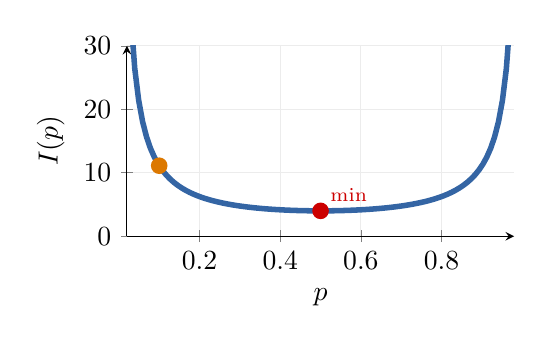
\begin{tikzpicture}
  \begin{axis}[
    width=6.5cm, height=4cm,
    xlabel={$p$},
    ylabel={$I(p)$},
    xmin=0.02, xmax=0.98,
    ymin=0, ymax=30,
    axis lines=left,
    grid=major, grid style={gray!15},
    every axis plot/.append style={line width=2pt, samples=100},
  ]
    \addplot[popblue, domain=0.02:0.98] {1/(x*(1-x))};
    \fill[sampred] (axis cs:0.5, 4) circle (3pt);
    \node[font=\scriptsize, sampred, above right] at (axis cs:0.5, 4) {min};
    \fill[orange1] (axis cs:0.1, 11.11) circle (3pt);
  \end{axis}
\end{tikzpicture}
\end{center}
\scriptsize\centering $p$ near 0 or 1: very informative. $p = 0.5$: max noise, min info.
\end{column}
\end{columns}
\end{frame}

\begin{frame}
\frametitle{Fisher Information: The Coin Flip Intuition}

\small
Why is $I(p) = \frac{1}{p(1-p)}$ shaped like a U?

\vspace{0.15cm}
\begin{columns}[T]
\begin{column}{0.48\textwidth}
\begin{center}
\textcolor{paramgreen}{\textbf{Biased coin ($p = 0.01$)}}

\vspace{0.1cm}
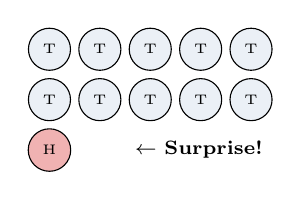
\begin{tikzpicture}[scale=0.8]
  \foreach \i in {1,...,10} {
    \node[circle, draw, fill=popblue!10, minimum size=0.5cm, font=\tiny] at ({mod(\i-1,5)*0.8}, {-floor((\i-1)/5)*0.8}) {T};
  }
  \node[circle, draw, fill=sampred!30, minimum size=0.5cm, font=\tiny] at (0, -1.6) {H};
  \node[font=\scriptsize, right] at (1.2, -1.6) {$\leftarrow$ \textbf{Surprise!}};
\end{tikzpicture}

\vspace{0.1cm}
\scriptsize
Almost every flip is Tails.\\
Seeing Heads is \textbf{very surprising} ---\\
tells you a lot about $p$.\\[3pt]
$I(0.01) \approx 100$ \;\textcolor{paramgreen}{\textbf{high info}}
\end{center}
\end{column}
\begin{column}{0.48\textwidth}
\begin{center}
\textcolor{sampred}{\textbf{Fair coin ($p = 0.5$)}}

\vspace{0.1cm}
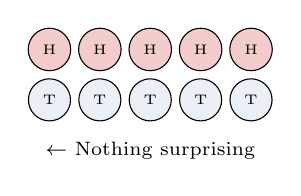
\begin{tikzpicture}[scale=0.8]
  \foreach \i in {1,...,5} {
    \node[circle, draw, fill=sampred!20, minimum size=0.5cm, font=\tiny] at ({(\i-1)*0.8}, 0) {H};
  }
  \foreach \i in {1,...,5} {
    \node[circle, draw, fill=popblue!10, minimum size=0.5cm, font=\tiny] at ({(\i-1)*0.8}, -0.8) {T};
  }
  \node[font=\scriptsize] at (1.6, -1.6) {$\leftarrow$ Nothing surprising};
\end{tikzpicture}

\vspace{0.1cm}
\scriptsize
H and T equally likely.\\
Neither outcome is surprising ---\\
each flip tells you \textbf{very little}.\\[3pt]
$I(0.5) = 4$ \;\textcolor{sampred}{\textbf{low info}}
\end{center}
\end{column}
\end{columns}

\vspace{0.2cm}
\begin{center}
\fcolorbox{popblue}{popblue!5}{\parbox{11cm}{\centering\small
  \textbf{Key insight:} Fisher information measures how \textbf{surprised} you are by the data.\\
  More surprise $=$ more information $=$ easier to pinpoint $\theta$.
}}
\end{center}
\end{frame}

% --- Item 13: Second derivative form ---
\begin{frame}
\frametitle{Fisher Information: Two Equivalent Forms}

\small
Under regularity conditions, there is an equivalent formula that's often easier to compute:

\vspace{0.1cm}
$$\boxed{I(\theta) = \mathbb{E}\!\left[s(\theta)^2\right] = -\mathbb{E}\!\left[\frac{\partial^2}{\partial\theta^2}\log f(X \mid \theta)\right]}$$

\vspace{0.05cm}
\textbf{Why are these the same?} Start from $\mathbb{E}[s(\theta)] = 0$ and differentiate both sides w.r.t.\ $\theta$:
$$0 = \frac{\partial}{\partial\theta}\mathbb{E}[s] = \mathbb{E}\!\left[\frac{\partial s}{\partial\theta}\right] + \mathbb{E}\!\left[s \cdot s\right] = \mathbb{E}[\ell''] + \mathbb{E}[s^2]$$

\vspace{-0.1cm}
So: $\;\mathbb{E}[s^2] = -\mathbb{E}[\ell'']$. \;\textcolor{paramgreen}{$\checkmark$}

\vspace{0.15cm}
\textbf{Verify for Bernoulli:} $\;\ell(p) = x\log p + (1{-}x)\log(1{-}p)$
$$\ell''(p) = -\frac{x}{p^2} - \frac{1-x}{(1-p)^2} \quad\Rightarrow\quad -\mathbb{E}[\ell''] = \frac{p}{p^2} + \frac{1-p}{(1-p)^2} = \frac{1}{p} + \frac{1}{1-p} = \frac{1}{p(1-p)} \;\;\textcolor{paramgreen}{\checkmark}$$
\end{frame}

% --- Item 14: Fix title overlap ---
\begin{frame}
\frametitle{Intuition: Sharp vs Flat Log-Likelihood}
\begin{center}
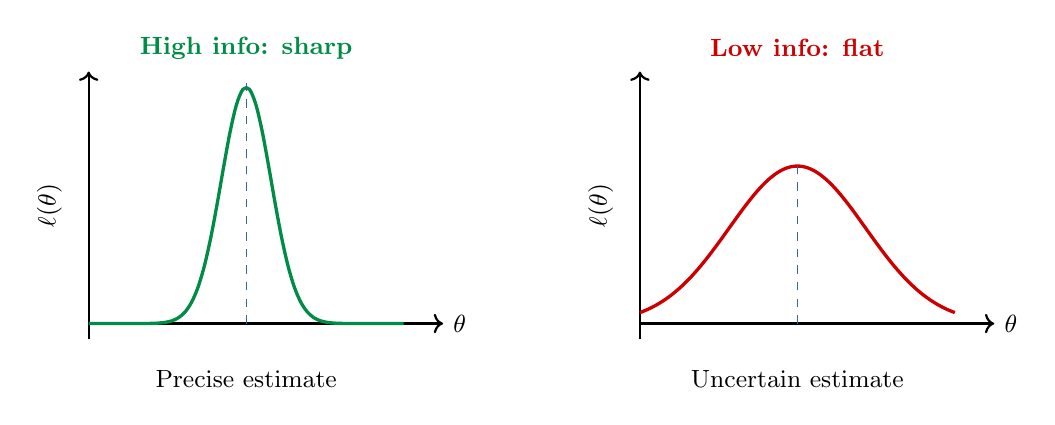
\begin{tikzpicture}
  % High information
  \begin{scope}[xshift=-5cm]
    \draw[thick, ->] (0, 0) -- (4.5, 0) node[right, font=\small] {$\theta$};
    \draw[thick, ->] (0, -0.2) -- (0, 3.2);
    \node[font=\small, rotate=90] at (-0.5, 1.5) {$\ell(\theta)$};
    \draw[very thick, paramgreen, smooth, domain=0:4, samples=50]
      plot (\x, {3*exp(-(\x-2)*(\x-2)/0.2)});
    \draw[dashed, popblue] (2, 0) -- (2, 3.1);
    \node[font=\small\bfseries, paramgreen] at (2, 3.5) {High info: sharp};
    \node[font=\small] at (2, -0.7) {Precise estimate};
  \end{scope}

  % Low information
  \begin{scope}[xshift=2cm]
    \draw[thick, ->] (0, 0) -- (4.5, 0) node[right, font=\small] {$\theta$};
    \draw[thick, ->] (0, -0.2) -- (0, 3.2);
    \node[font=\small, rotate=90] at (-0.5, 1.5) {$\ell(\theta)$};
    \draw[very thick, sampred, smooth, domain=0:4, samples=50]
      plot (\x, {2*exp(-(\x-2)*(\x-2)/1.5)});
    \draw[dashed, popblue] (2, 0) -- (2, 2.1);
    \node[font=\small\bfseries, sampred] at (2, 3.5) {Low info: flat};
    \node[font=\small] at (2, -0.7) {Uncertain estimate};
  \end{scope}
\end{tikzpicture}
\end{center}

\vspace{0.2cm}
\begin{center}
\small $I(\theta)$ measures the \textbf{curvature} of the log-likelihood at the true $\theta$.\\[4pt]
Sharp curve $\Rightarrow$ high $I(\theta)$ $\Rightarrow$ data is very informative $\Rightarrow$ estimator is precise.\\[4pt]
This connects the two forms: $I(\theta) = -\mathbb{E}[\ell'']$ is literally the expected curvature.
\end{center}
\end{frame}

% --- Item 15: Cramér-Rao in 2 slides ---
\begin{frame}
\frametitle{Cram\'er--Rao Lower Bound}

\small
Now we can answer the fundamental question. For any \textbf{unbiased} estimator $\hat\theta$ based on $n$ i.i.d.\ observations:

$$\boxed{\text{Var}(\hat\theta) \;\geq\; \frac{1}{n \cdot I(\theta)}}$$

\vspace{0.1cm}
\textbf{Intuition:} Why $\frac{1}{n \cdot I(\theta)}$?
\begin{itemize}\setlength{\itemsep}{3pt}
  \item \textbf{More observations ($n$ large)} $\Rightarrow$ bound gets smaller $\Rightarrow$ can estimate more precisely
  \item \textbf{More informative data ($I(\theta)$ large)} $\Rightarrow$ bound gets smaller $\Rightarrow$ each observation tells us more
  \item The bound is \textbf{tight} for many models --- it's the actual achievable precision
\end{itemize}

\pause
\vspace{0.15cm}
\textbf{Verify for Bernoulli:}

\vspace{-0.1cm}
\begin{center}
\small
$I(p) = \frac{1}{p(1-p)}$ \quad$\Rightarrow$\quad CR bound: $\text{Var}(\hat{p}) \geq \frac{1}{n \cdot \frac{1}{p(1-p)}} = \frac{p(1-p)}{n}$

\vspace{0.1cm}
Actual variance of $\hat{p} = \bar{X}$: $\;\text{Var}(\hat{p}) = \frac{p(1-p)}{n}$ \;\;\textcolor{paramgreen}{$\checkmark$ Hits the bound exactly!}
\end{center}
\end{frame}

\begin{frame}
\frametitle{Cram\'er--Rao: Efficiency and Practical Use}

\begin{center}
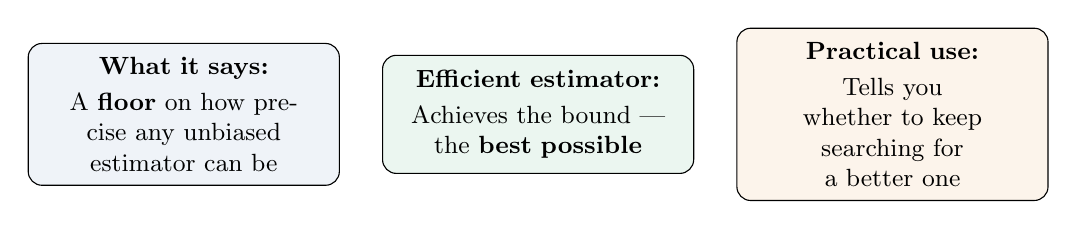
\begin{tikzpicture}[
  cbox/.style={draw, rounded corners=5pt, minimum width=3.8cm, minimum height=1.5cm, align=center, text width=3.6cm, inner sep=5pt, font=\small}
]
  \node[cbox, fill=popblue!8] at (-4.5, 0) {
    \textbf{What it says:}\\[2pt]
    A \textbf{floor} on how precise any unbiased estimator can be
  };
  \node[cbox, fill=paramgreen!8] at (0, 0) {
    \textbf{Efficient estimator:}\\[2pt]
    Achieves the bound ---\\
    the \textbf{best possible}
  };
  \node[cbox, fill=orange1!8] at (4.5, 0) {
    \textbf{Practical use:}\\[2pt]
    Tells you whether to keep\\
    searching for a better one
  };
\end{tikzpicture}
\end{center}

\vspace{0.2cm}
\begin{center}
\footnotesize
\renewcommand{\arraystretch}{1.8}
\begin{tabular}{@{}lcccc@{}}
  \textbf{Model} & \textbf{Estimator} & $\text{Var}(\hat\theta)$ & \textbf{CR bound} & \textbf{Efficient?} \\
  \hline
  $\text{Bern}(p)$ & $\hat{p} = \bar{X}$ & $\frac{p(1-p)}{n}$ & $\frac{p(1-p)}{n}$ & \textcolor{paramgreen}{\textbf{Yes}} \\
  $N(\mu, \sigma^2_0)$ & $\hat\mu = \bar{X}$ & $\frac{\sigma^2_0}{n}$ & $\frac{\sigma^2_0}{n}$ & \textcolor{paramgreen}{\textbf{Yes}} \\
  $\text{Exp}(\lambda)$ & $\hat\lambda = 1/\bar{X}$ & $\frac{\lambda^2}{n}$ & $\frac{\lambda^2}{n}$ & \textcolor{paramgreen}{\textbf{Yes}} \\
  \hline
\end{tabular}
\end{center}
\end{frame}

% --- Regularity conditions: Slide 1 ---
\begin{frame}
\frametitle{Regularity Conditions: When Does CR Apply?}

\small
The Cram\'er--Rao bound doesn't hold for \emph{every} model. It requires these \textbf{regularity conditions}:

\vspace{0.2cm}
\begin{enumerate}\setlength{\itemsep}{6pt}
  \item \textbf{Fixed support:} the set of $x$ values where $f(x \mid \theta) > 0$ doesn't depend on $\theta$
  \item \textbf{Interior parameter:} $\theta$ is in the \textbf{interior} of the parameter space (not at a boundary)
  \item \textbf{Differentiation under the integral:} we can swap $\frac{\partial}{\partial\theta}$ and $\int$ \\
    \small (this is how we proved $\mathbb{E}[s(\theta)] = 0$ and derived the two forms of $I(\theta)$)
  \item \textbf{Finite information:} $0 < I(\theta) < \infty$
\end{enumerate}

\vspace{0.3cm}
\begin{center}
\fcolorbox{paramgreen}{paramgreen!5}{\parbox{11cm}{\centering\small
  \textbf{Good news:} All \textbf{exponential family} distributions (Normal, Bernoulli, Poisson, Exponential, Gamma, \ldots) automatically satisfy these conditions. The CR bound always applies to them.
}}
\end{center}
\end{frame}

% --- Regularity conditions: Slide 2 (counterexample) ---
\begin{frame}
\frametitle{When CR Fails: The Uniform Distribution}

\small
\textbf{Counterexample:} $X_1, \ldots, X_n \sim \text{Uniform}(0, \theta)$

\vspace{0.1cm}
\begin{columns}[T]
\begin{column}{0.48\textwidth}
\begin{itemize}\setlength{\itemsep}{4pt}
  \item Support is $[0, \theta]$ --- depends on $\theta$!\\(violates condition \#1)
  \item The sufficient statistic is $X_{(n)} = \max_i X_i$
  \item Its variance: $\text{Var}(X_{(n)}) \sim \frac{1}{n^2}$
\end{itemize}

\vspace{0.1cm}
\fcolorbox{warnred}{warnred!5}{\parbox{5.5cm}{\centering\small
  CR would predict a floor of $1/n$.\\
  But $1/n^2$ is \textbf{much faster} --- we beat the ``bound''!\\[2pt]
  The bound simply \textbf{doesn't apply} here.
}}
\end{column}
\begin{column}{0.48\textwidth}
\begin{center}
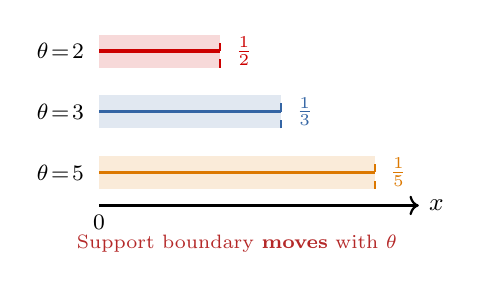
\begin{tikzpicture}[scale=0.7]
  % theta = 2 (RED - top of Armenian flag)
  \fill[sampred!15] (0, 2.2) rectangle (2.2, 2.8);
  \draw[very thick, sampred] (0, 2.5) -- (2.2, 2.5);
  \draw[thick, sampred, dashed] (2.2, 2.2) -- (2.2, 2.8);
  \node[left, font=\footnotesize] at (-0.1, 2.5) {$\theta\!=\!2$};
  \node[right, font=\footnotesize, sampred] at (2.3, 2.5) {$\frac{1}{2}$};

  % theta = 3 (BLUE - middle of Armenian flag)
  \fill[popblue!15] (0, 1.1) rectangle (3.3, 1.7);
  \draw[very thick, popblue] (0, 1.4) -- (3.3, 1.4);
  \draw[thick, popblue, dashed] (3.3, 1.1) -- (3.3, 1.7);
  \node[left, font=\footnotesize] at (-0.1, 1.4) {$\theta\!=\!3$};
  \node[right, font=\footnotesize, popblue] at (3.4, 1.4) {$\frac{1}{3}$};

  % theta = 5 (ORANGE - bottom of Armenian flag)
  \fill[orange1!15] (0, 0) rectangle (5.0, 0.6);
  \draw[very thick, orange1] (0, 0.3) -- (5.0, 0.3);
  \draw[thick, orange1, dashed] (5.0, 0) -- (5.0, 0.6);
  \node[left, font=\footnotesize] at (-0.1, 0.3) {$\theta\!=\!5$};
  \node[right, font=\footnotesize, orange1] at (5.1, 0.3) {$\frac{1}{5}$};

  % x-axis
  \draw[thick, ->] (0, -0.3) -- (5.8, -0.3) node[right, font=\small] {$x$};
  \node[below, font=\footnotesize] at (0, -0.3) {$0$};

  \node[font=\scriptsize, warnred, text width=4.5cm, align=center] at (2.5, -1.0) {Support boundary \textbf{moves} with $\theta$};
\end{tikzpicture}
\end{center}
\end{column}
\end{columns}

\vspace{0.15cm}
\centering\small\textbf{Lesson:} Always check regularity conditions before applying CR.\\
When they fail, estimators can be \emph{better} than the ``bound'' suggests.
\end{frame}

% ============================================================
\section{Admissibility and Minimax}

\begin{frame}
\frametitle{Beyond Unbiasedness: What If We Allow Bias?}

\small
The Cram\'er--Rao bound tells us: among \textbf{unbiased} estimators, variance $\geq \frac{1}{nI(\theta)}$.

\vspace{0.2cm}
But from Lecture~3, we know biased estimators can have \textbf{lower MSE}!

\vspace{0.15cm}
\begin{center}
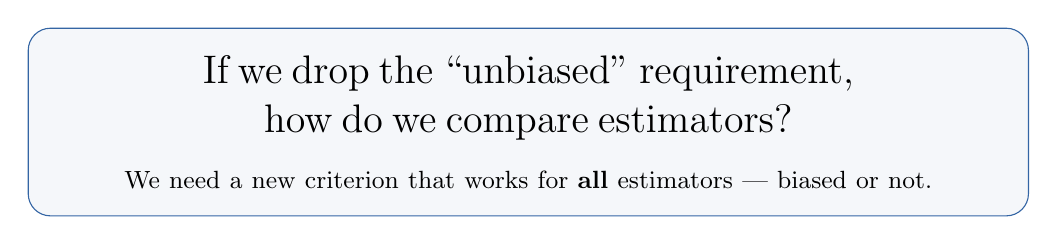
\begin{tikzpicture}
  \node[draw=popblue, fill=popblue!5, rounded corners=8pt, text width=12cm, align=center, inner sep=10pt] {
    {\Large If we drop the ``unbiased'' requirement,\\[4pt]
    how do we compare estimators?}\\[8pt]
    \small We need a new criterion that works for \textbf{all} estimators --- biased or not.
  };
\end{tikzpicture}
\end{center}

\vspace{0.2cm}
\begin{center}
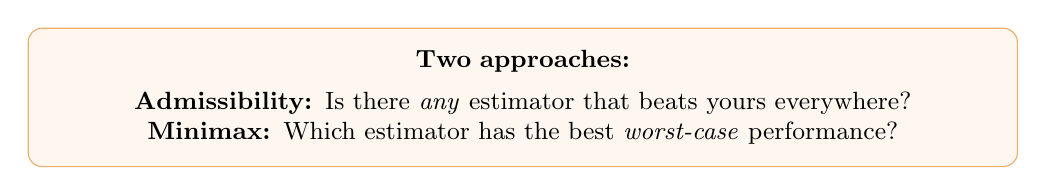
\begin{tikzpicture}
  \node[draw=orange1!60, fill=orange1!6, rounded corners=5pt, text width=12cm, align=center, inner sep=8pt, font=\small] {
    \textbf{Two approaches:}\\[4pt]
    \textbf{Admissibility:} Is there \emph{any} estimator that beats yours everywhere?\\
    \textbf{Minimax:} Which estimator has the best \emph{worst-case} performance?
  };
\end{tikzpicture}
\end{center}
\end{frame}

\begin{frame}
\frametitle{Admissibility}

\small
\textbf{Definition:} $\hat\theta_1$ is \textbf{inadmissible} if $\exists\;\hat\theta_2$ that \textbf{dominates} it:
\vspace{-0.2cm}
$$\text{MSE}(\hat\theta_2, \theta) \leq \text{MSE}(\hat\theta_1, \theta) \;\;\forall\,\theta, \quad\text{with strict inequality for some } \theta$$

\vspace{-0.2cm}
An estimator is \textbf{admissible} if no other estimator dominates it.

\pause
\vspace{-0.05cm}
\begin{center}
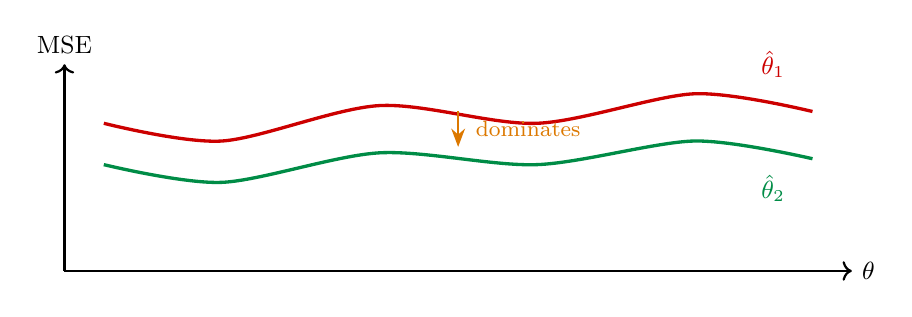
\begin{tikzpicture}[yscale=0.75]
  \draw[thick, ->] (0, 0) -- (10, 0) node[right, font=\small] {$\theta$};
  \draw[thick, ->] (0, 0) -- (0, 3.5) node[above, font=\small] {MSE};

  \draw[very thick, sampred, smooth] plot coordinates {
    (0.5, 2.5) (2, 2.2) (4, 2.8) (6, 2.5) (8, 3.0) (9.5, 2.7)
  };
  \node[font=\small\bfseries, sampred] at (9, 3.5) {$\hat\theta_1$};

  \draw[very thick, paramgreen, smooth] plot coordinates {
    (0.5, 1.8) (2, 1.5) (4, 2.0) (6, 1.8) (8, 2.2) (9.5, 1.9)
  };
  \node[font=\small\bfseries, paramgreen] at (9, 1.4) {$\hat\theta_2$};

  \draw[-{Stealth}, thick, orange1] (5, 2.7) -- (5, 2.1);
  \node[font=\footnotesize, orange1, right] at (5.1, 2.4) {dominates};
\end{tikzpicture}
\end{center}

\vspace{-0.15cm}
\small $\hat\theta_1$ is \textbf{inadmissible} --- $\hat\theta_2$ is at least as good everywhere, and strictly better somewhere.

\vspace{0.05cm}
\begin{center}
\fcolorbox{violet1}{violet1!5}{\parbox{12cm}{\centering\small
  \textbf{Familiar?} This is exactly \textbf{Pareto dominance} from multi-criteria optimization!\\[1pt]
  $\hat\theta_2$ Pareto-dominates $\hat\theta_1$: better on some criteria (values of $\theta$), no worse on any.\\
  Admissible estimators $=$ the \textbf{Pareto front} of the MSE landscape.
}}
\end{center}
\end{frame}

% --- What is shrinkage? ---
\begin{frame}
\frametitle{What Is Shrinkage?}

\small
\textbf{Idea:} Instead of using the raw estimate, \textbf{pull it toward a fixed target} (often $0$ or the grand mean).

\vspace{0.15cm}
\begin{center}
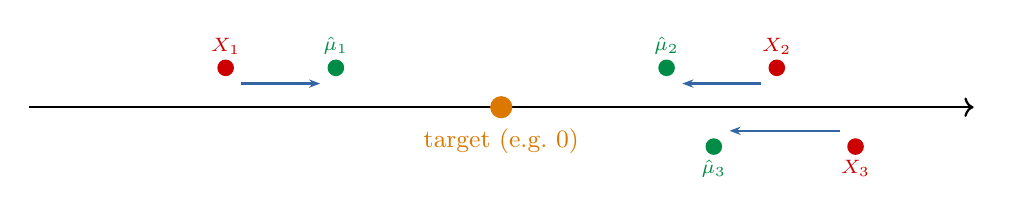
\begin{tikzpicture}
  \draw[thick, ->] (-1, 0) -- (11, 0) node[right, font=\small] {};

  % Target
  \fill[orange1] (5, 0) circle (4pt);
  \node[below, font=\small, orange1] at (5, -0.15) {target (e.g.\ $0$)};

  % Raw estimates and shrunk versions
  \fill[sampred] (1.5, 0.5) circle (3pt);
  \node[above, font=\scriptsize, sampred] at (1.5, 0.55) {$X_1$};
  \fill[paramgreen] (2.9, 0.5) circle (3pt);
  \node[above, font=\scriptsize, paramgreen] at (2.9, 0.55) {$\hat\mu_1$};
  \draw[-{Stealth[length=4pt]}, popblue, thick] (1.7, 0.3) -- (2.7, 0.3);

  \fill[sampred] (8.5, 0.5) circle (3pt);
  \node[above, font=\scriptsize, sampred] at (8.5, 0.55) {$X_2$};
  \fill[paramgreen] (7.1, 0.5) circle (3pt);
  \node[above, font=\scriptsize, paramgreen] at (7.1, 0.55) {$\hat\mu_2$};
  \draw[-{Stealth[length=4pt]}, popblue, thick] (8.3, 0.3) -- (7.3, 0.3);

  \fill[sampred] (9.5, -0.5) circle (3pt);
  \node[below, font=\scriptsize, sampred] at (9.5, -0.55) {$X_3$};
  \fill[paramgreen] (7.7, -0.5) circle (3pt);
  \node[below, font=\scriptsize, paramgreen] at (7.7, -0.55) {$\hat\mu_3$};
  \draw[-{Stealth[length=4pt]}, popblue, thick] (9.3, -0.3) -- (7.9, -0.3);
\end{tikzpicture}
\end{center}

\vspace{0.1cm}
The shrinkage estimator has the form: $\;\hat\mu_i^{\text{shrunk}} = (1 - c) \cdot X_i + c \cdot \text{target}, \quad 0 < c < 1$

\pause
\vspace{0.15cm}
\textbf{Why does this help?}
\begin{itemize}\setlength{\itemsep}{2pt}
  \item Raw estimates $X_i$ are \textbf{noisy} --- they overshoot in random directions
  \item Pulling toward a target \textbf{cancels some noise} (reduces variance)
  \item Yes, it introduces \textbf{bias} --- but the variance reduction can more than compensate
  \item Net effect: \textbf{lower MSE} $=$ Bias$^2$ + Var (the bias-variance tradeoff!)
\end{itemize}
\end{frame}

% --- Stein's Paradox: Slide 1 (the paradox) ---
\begin{frame}
\frametitle{Stein's Paradox (1956)}

\small
\textbf{Setup:} Estimate $d$ \textbf{unrelated} means simultaneously.
One noisy measurement each: $X_i \sim N(\mu_i, 1)$.

\vspace{0.05cm}
\footnotesize
\quad $\mu_1 =$ avg temperature in Yerevan, \;$\mu_2 =$ price of tea in China, \;$\mu_3 =$ height of Eiffel Tower

\pause
\vspace{0.1cm}
\small
\begin{center}
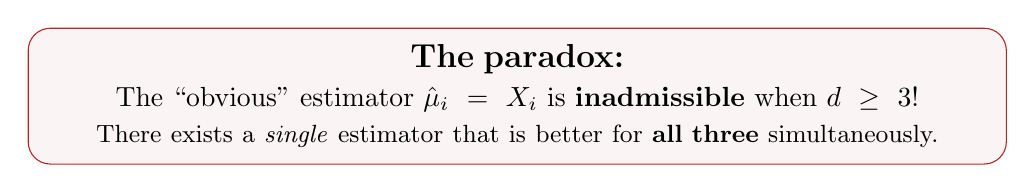
\begin{tikzpicture}
  \node[draw=warnred, fill=warnred!5, rounded corners=8pt, text width=12cm, align=center, inner sep=6pt] {
    {\large\bfseries The paradox:}\\[2pt]
    The ``obvious'' estimator $\hat\mu_i = X_i$ is \textbf{inadmissible} when $d \geq 3$!\\[1pt]
    \small There exists a \emph{single} estimator that is better for \textbf{all three} simultaneously.
  };
\end{tikzpicture}
\end{center}

\pause
\vspace{0.05cm}
The \textbf{James--Stein estimator} shrinks every $X_i$ toward zero:
$$\hat\mu_i^{\,JS} = \underbrace{\left(1 - \frac{d-2}{\|\mathbf{X}\|^2}\right)}_{\text{shrinkage factor } c}\! \cdot\, X_i$$

\vspace{-0.2cm}
\centering\small
Why is this shocking? These quantities are \textbf{completely unrelated}!\\
Yet estimating them \textbf{jointly} beats estimating each one separately.
\end{frame}

% --- Stein's Paradox: Slide 2 (why it works + visual) ---
\begin{frame}
\frametitle{Why Does Stein's Paradox Work?}

\vspace{-0.1cm}
\begin{columns}[T]
\begin{column}{0.48\textwidth}
\small
\textbf{The MSE comparison:}
\begin{itemize}\setlength{\itemsep}{3pt}
  \item Raw: total MSE $= d$ \;{\scriptsize ($1$ per coordinate)}
  \item James--Stein: total MSE $< d$\\{\scriptsize (provably, for \emph{any} $\boldsymbol{\mu}$, when $d \geq 3$)}
\end{itemize}

\vspace{0.1cm}
\textbf{Why $d \geq 3$?}
\begin{itemize}\setlength{\itemsep}{2pt}
  \footnotesize
  \item The shrinkage factor $c = 1 - \frac{d-2}{\|\mathbf{X}\|^2}$ must be estimated from data
  \item In $d = 1, 2$: estimating $c$ is too noisy --- the error wipes out the gain
  \item In $d \geq 3$: $\|\mathbf{X}\|^2$ concentrates enough $\to$ net win
\end{itemize}
\end{column}
\begin{column}{0.48\textwidth}
\begin{center}
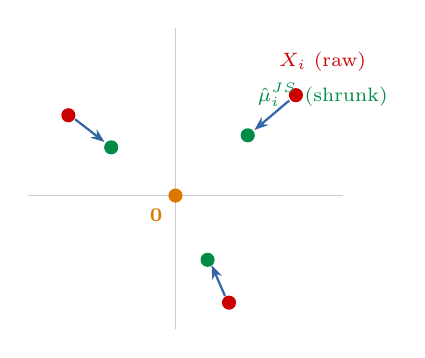
\begin{tikzpicture}[scale=0.85]
  \draw[gray!40, thin] (-2.2, 0) -- (2.5, 0);
  \draw[gray!40, thin] (0, -2.0) -- (0, 2.5);
  \fill[orange1] (0, 0) circle (3pt);
  \node[font=\scriptsize, orange1, below left] at (-0.05, -0.05) {$\mathbf{0}$};

  % Point 1
  \fill[sampred] (1.8, 1.5) circle (3pt);
  \fill[paramgreen] (1.08, 0.9) circle (3pt);
  \draw[-{Stealth[length=5pt]}, popblue, thick] (1.7, 1.42) -- (1.18, 0.98);

  % Point 2
  \fill[sampred] (-1.6, 1.2) circle (3pt);
  \fill[paramgreen] (-0.96, 0.72) circle (3pt);
  \draw[-{Stealth[length=5pt]}, popblue, thick] (-1.5, 1.14) -- (-1.06, 0.8);

  % Point 3
  \fill[sampred] (0.8, -1.6) circle (3pt);
  \fill[paramgreen] (0.48, -0.96) circle (3pt);
  \draw[-{Stealth[length=5pt]}, popblue, thick] (0.74, -1.5) -- (0.54, -1.04);

  \node[font=\scriptsize, sampred] at (2.2, 2.0) {$X_i$ (raw)};
  \node[font=\scriptsize, paramgreen] at (2.2, 1.5) {$\hat\mu_i^{JS}$ (shrunk)};
\end{tikzpicture}
\end{center}

\scriptsize\centering
Each arrow shrinks toward $\mathbf{0}$.\\
On average, the shrunk points are\\
\textbf{closer to the true} $\boldsymbol{\mu}$.
\end{column}
\end{columns}

\vspace{0.05cm}
\begin{center}
\fcolorbox{violet1}{violet1!5}{\parbox{12cm}{\centering\small
  \textbf{Connection to ML:} James--Stein is an early form of \textbf{regularization}.
  Ridge regression ($L^2$ penalty) does exactly this: shrink coefficients toward zero.
}}
\end{center}
\end{frame}

\begin{frame}
\frametitle{Minimax Estimators}

\small
\textbf{Analogy:} You don't know tomorrow's weather ($\theta$).
A minimax thinker picks the option whose \textbf{worst outcome is least bad}.

\vspace{0.05cm}
A \textbf{minimax} estimator minimizes the \textbf{worst-case} risk:
\vspace{-0.15cm}
$$\hat\theta_{\text{minimax}} = \arg\min_{\hat\theta}\; \max_{\theta}\; \text{MSE}(\hat\theta, \theta)$$

\vspace{-0.35cm}
\begin{center}
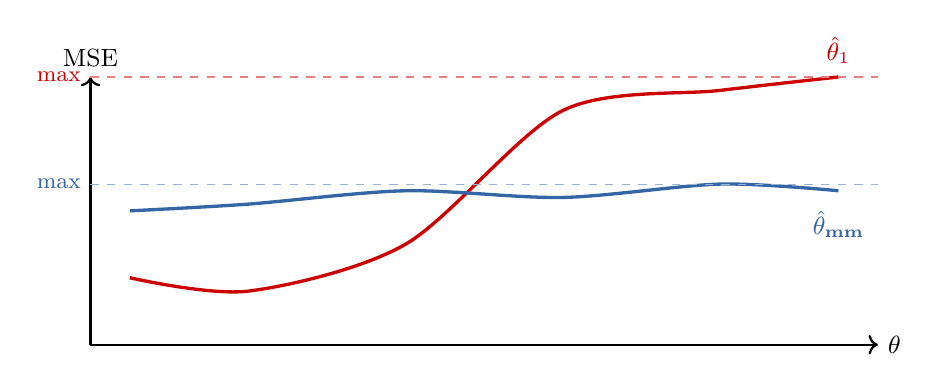
\begin{tikzpicture}[yscale=0.85]
  \draw[thick, ->] (0, 0) -- (10, 0) node[right, font=\small] {$\theta$};
  \draw[thick, ->] (0, 0) -- (0, 4) node[above, font=\small] {MSE};

  \draw[very thick, sampred, smooth] plot coordinates {
    (0.5, 1.0) (2, 0.8) (4, 1.5) (6, 3.5) (8, 3.8) (9.5, 4.0)
  };
  \node[font=\small\bfseries, sampred] at (9.5, 4.4) {$\hat\theta_1$};
  \draw[dashed, sampred!50] (0, 4.0) -- (10, 4.0);
  \node[left, font=\footnotesize, sampred] at (0, 4.0) {max};

  \draw[very thick, popblue, smooth] plot coordinates {
    (0.5, 2.0) (2, 2.1) (4, 2.3) (6, 2.2) (8, 2.4) (9.5, 2.3)
  };
  \node[font=\small\bfseries, popblue] at (9.5, 1.8) {$\hat\theta_{\text{mm}}$};
  \draw[dashed, popblue!50] (0, 2.4) -- (10, 2.4);
  \node[left, font=\footnotesize, popblue] at (0, 2.4) {max};
\end{tikzpicture}
\end{center}

\vspace{-0.2cm}
\begin{center}
\small $\hat\theta_1$ can be great for some $\theta$, but terrible for others.
$\hat\theta_{\text{mm}}$ is never great, but \textbf{never terrible either}.
\end{center}
\end{frame}

\begin{frame}
\frametitle{Three Philosophies of Estimation}
\begin{center}
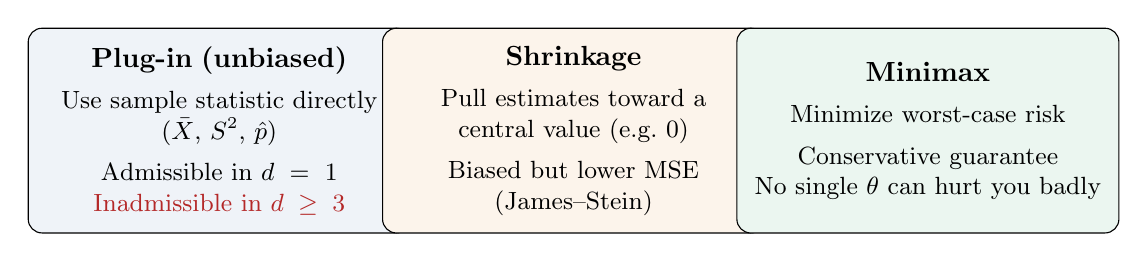
\begin{tikzpicture}[
  rbox/.style={draw, rounded corners=5pt, minimum width=4.8cm, minimum height=2.6cm, align=center, text width=4.5cm, inner sep=5pt, font=\small}
]
  \node[rbox, fill=popblue!8] at (-4.5, 0) {
    \textbf{\normalsize Plug-in (unbiased)}\\[4pt]
    Use sample statistic directly\\
    ($\bar{X}$, $S^2$, $\hat{p}$)\\[4pt]
    Admissible in $d = 1$\\
    \textcolor{warnred}{Inadmissible in $d \geq 3$}
  };
  \node[rbox, fill=orange1!8] at (0, 0) {
    \textbf{\normalsize Shrinkage}\\[4pt]
    Pull estimates toward a\\
    central value (e.g.\ $0$)\\[4pt]
    Biased but lower MSE\\
    (James--Stein)
  };
  \node[rbox, fill=paramgreen!8] at (4.5, 0) {
    \textbf{\normalsize Minimax}\\[4pt]
    Minimize worst-case risk\\[4pt]
    Conservative guarantee\\
    No single $\theta$ can hurt you badly
  };
\end{tikzpicture}
\end{center}

\vspace{0.2cm}
\begin{center}
\fcolorbox{violet1}{violet1!5}{\parbox{11cm}{\centering\small
  \textbf{Takeaway:} In high dimensions ($d \geq 3$), shrinkage estimators are provably better\\
  than using each sample statistic on its own. We'll see more of this in later lectures.
}}
\end{center}
\end{frame}

% ============================================================
\section{Summary}

% --- Item 18: What we haven't covered ---
\begin{frame}
\frametitle{What We Haven't Covered (Yet)}

\small
Lectures 3--4 focused on \textbf{point estimation} --- producing a single ``best guess'' for $\theta$.
But there's much more to statistical inference:

\vspace{0.1cm}
\begin{center}
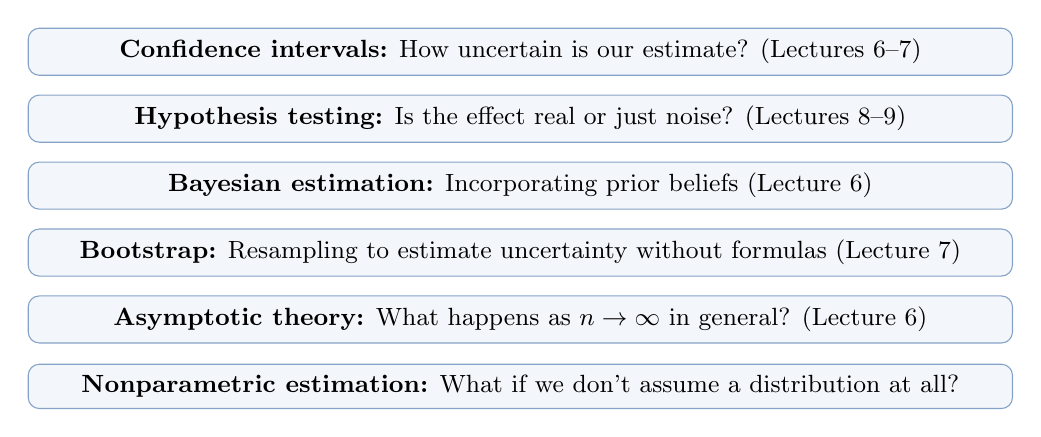
\begin{tikzpicture}[
  fbox/.style={draw=popblue!60, fill=popblue!6, rounded corners=4pt, minimum width=12.5cm, align=left, inner sep=4pt, font=\small}
]
  \node[fbox] at (0, 2.15) {\textbf{Confidence intervals:} How uncertain is our estimate? (Lectures 6--7)};
  \node[fbox] at (0, 1.3) {\textbf{Hypothesis testing:} Is the effect real or just noise? (Lectures 8--9)};
  \node[fbox] at (0, 0.45) {\textbf{Bayesian estimation:} Incorporating prior beliefs (Lecture 6)};
  \node[fbox] at (0, -0.4) {\textbf{Bootstrap:} Resampling to estimate uncertainty without formulas (Lecture 7)};
  \node[fbox] at (0, -1.25) {\textbf{Asymptotic theory:} What happens as $n \to \infty$ in general? (Lecture 6)};
  \node[fbox] at (0, -2.1) {\textbf{Nonparametric estimation:} What if we don't assume a distribution at all?};
\end{tikzpicture}
\end{center}

\vspace{0.05cm}
\centering\small Our tools (bias, MSE, CR bound, sufficiency) will be the \textbf{foundation} for all of these.
\end{frame}

\begin{frame}
\frametitle{Summary: How to Judge an Estimator}
\begin{center}
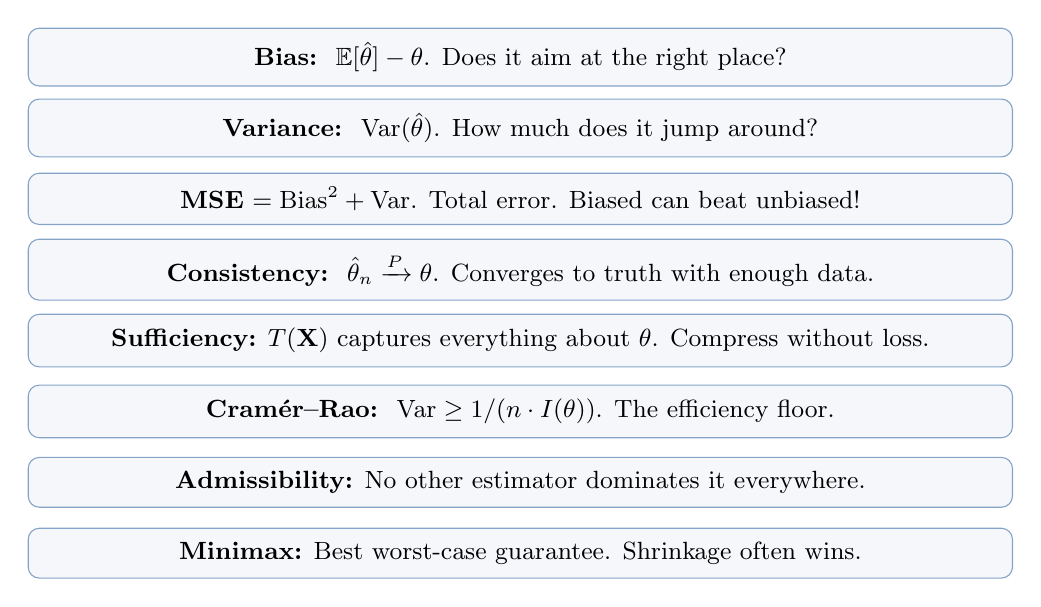
\begin{tikzpicture}[
  sbox/.style={draw=popblue!60, fill=popblue!5, rounded corners=4pt, minimum width=12.5cm, minimum height=0.6cm, align=left, inner sep=5pt, font=\small}
]
  \node[sbox] at (0, 3.15) {\textbf{Bias:} $\;\mathbb{E}[\hat\theta] - \theta$. Does it aim at the right place?};
  \node[sbox] at (0, 2.25) {\textbf{Variance:} $\;\text{Var}(\hat\theta)$. How much does it jump around?};
  \node[sbox] at (0, 1.35) {\textbf{MSE} $= \text{Bias}^2 + \text{Var}$. Total error. Biased can beat unbiased!};
  \node[sbox] at (0, 0.45) {\textbf{Consistency:} $\;\hat\theta_n \xrightarrow{P} \theta$. Converges to truth with enough data.};
  \node[sbox] at (0, -0.45) {\textbf{Sufficiency:} $T(\mathbf{X})$ captures everything about $\theta$. Compress without loss.};
  \node[sbox] at (0, -1.35) {\textbf{Cram\'er--Rao:} $\;\text{Var} \geq 1/(n \cdot I(\theta))$. The efficiency floor.};
  \node[sbox] at (0, -2.25) {\textbf{Admissibility:} No other estimator dominates it everywhere.};
  \node[sbox] at (0, -3.15) {\textbf{Minimax:} Best worst-case guarantee. Shrinkage often wins.};
\end{tikzpicture}
\end{center}
\end{frame}

\begin{frame}
\frametitle{Homework}
\begin{enumerate}
  \item Compute the Fisher information $I(\lambda)$ for $\text{Poisson}(\lambda)$.\\
    Find the Cram\'er--Rao lower bound for estimating $\lambda$.
    Is $\hat\lambda = \bar{X}$ efficient?

  \vspace{0.15cm}
  \item For $X_1, \ldots, X_n \sim \text{Exp}(\lambda)$: compute $I(\lambda)$ using both\\
    the variance-of-score and second-derivative formulas. Verify they agree.

  \vspace{0.15cm}
  \item Three estimators $T_1, T_2, T_3$ have MSE curves as functions of $\theta \in [0,1]$.\\
    Sketch an example where $T_1$ and $T_2$ are admissible but $T_3$ is not.\\
    Then sketch an example where $T_1$ is the minimax estimator.
\end{enumerate}
\end{frame}

\begin{frame}
\begin{center}
  {\Huge\bfseries\textcolor{popblue}{Questions?}}
\end{center}
\end{frame}

\end{document}
